\documentclass[11pt,letterpaper]{article}

% ---------------------------------------------------------------------------
% Diffuse RAFs and productive operation:
% asymptotic singleton dominance in a random polymer model.
%
% Author metadata: set the macros below before submission.  The companion
% separation-theorem manuscript is cited through \CompanionAuthor.
% ---------------------------------------------------------------------------
\newcommand{\PaperAuthor}{Author name to be inserted}
\newcommand{\PaperAffiliation}{Affiliation to be inserted}
\newcommand{\PaperDate}{14 September 2026}
\newcommand{\CompanionAuthor}{Author name to be inserted}

\usepackage[T1]{fontenc}
\usepackage[utf8]{inputenc}
\usepackage{lmodern}
\usepackage{microtype}
\usepackage[letterpaper,margin=1in]{geometry}
\usepackage{amsmath,amssymb,amsthm,mathtools}
\usepackage{booktabs,array,longtable}
\usepackage{enumitem}
\usepackage{xcolor}
\usepackage{tikz}
\usetikzlibrary{arrows.meta,positioning,calc,shapes.misc}
\usepackage[obeyspaces,spaces]{url}
\usepackage[numbers,sort&compress]{natbib}
\usepackage[colorlinks=true,linkcolor=blue!50!black,citecolor=blue!50!black,urlcolor=blue!50!black]{hyperref}
\hypersetup{pdftitle={Diffuse RAFs and productive operation: asymptotic singleton dominance in a random polymer model},
  pdfkeywords={autocatalytic sets, RAF, binary polymer model, power-law catalysis, stochastic mass action, rare events, minimum RAF, Lean 4}}

%% Breakable typewriter identifiers for Lean names: \lean{Foo.bar_baz}
%% (url-style command: write underscores unescaped; never use inside \caption)
\DeclareUrlCommand\lean{\urlstyle{tt}}

\setlist{itemsep=2pt,topsep=3pt}
\setlength{\emergencystretch}{2em}

\theoremstyle{plain}
\newtheorem{theorem}{Theorem}[section]
\newtheorem{proposition}[theorem]{Proposition}
\newtheorem{lemma}[theorem]{Lemma}
\newtheorem{corollary}[theorem]{Corollary}
\theoremstyle{definition}
\newtheorem{definition}[theorem]{Definition}
\theoremstyle{remark}
\newtheorem{remark}[theorem]{Remark}
\numberwithin{equation}{section}

\newcommand{\PP}{\mathbb P}
\newcommand{\EE}{\mathbb E}
\newcommand{\R}{\mathbb R}
\newcommand{\XX}{\mathcal X}
\newcommand{\RR}{\mathcal R}
\newcommand{\cF}{\mathcal F}
\newcommand{\cT}{\mathcal T}
\newcommand{\cG}{\mathcal G}
\newcommand{\cI}{\mathcal I}
\newcommand{\eps}{\varepsilon}
\newcommand{\ind}{\mathbf 1}
\newcommand{\cl}{\operatorname{cl}}
\newcommand{\m}{\mathsf m}
\newcommand{\dd}{\,\mathrm d}
\newcommand{\loc}{\mathrm{loc}}
\newcommand{\oth}{\mathrm{other}}
\newcommand{\del}{\mathrm{del}}
\newcommand{\thetaq}{\theta(q_*)}

\title{Diffuse RAFs and productive operation:\\ asymptotic singleton dominance\\ in a random polymer model}
\author{\PaperAuthor\\[2pt]\small\PaperAffiliation}
\date{\PaperDate}

\begin{document}
\maketitle

\begin{abstract}
A reflexively autocatalytic and food-generated set (RAF) certifies that a reaction network can regenerate its own catalysts from food. In the capped-Zipf binary polymer model at the critical exponent sequence $a_n=2-2/n$, a companion paper proved that RAFs exist with limiting probability $\theta(q_*)\in(0,1)$, that the minimum RAF size is subexponential given existence, and that a fed, diluted stochastic mass-action reactor started from food exports a fixed amount of nonfood polymer during a fixed window with probability of order $p_n\asymp2^{-n}$, the probability that one specified molecule catalyzes one specified reaction. It left open whether the rare productive realizations typically rely on a diffuse collective organization or contain a one-channel RAF. We prove the latter. At a sufficient quadratic volume scale, the probability of productive output without a productive one-channel incidence is $o(p_n)$; hence, conditional on productive output, the minimum RAF size converges to one, with or without conditioning on RAF existence. The proof combines a uniform kinetic exclusion, valid pointwise in every catalytic environment with at most one incidence in a fixed local rectangle, with an exact rare-multiplicity estimate for the heavy-tailed source that retains the dependence between assignments of one catalyst. The kinetic exclusion rests on two observables: a conserved product credit that cancels a mixed food--nonfood channel exactly, and a washout penalty that lets the dilution of an outsider catalyst pay for the material it could amplify. Consequences identify a unique short catalytic nucleus under successful-run conditioning and among environments with any fixed positive reliability, show that deleting that incidence makes the output probability exponentially small, and show that its signed catalytic input supplies more than three quarters of the measured export. Exactly $224$ productive candidate incidences give the asymptotic upper prefactor $224$ for the success probability. In contrast, the minimum RAF size diverges in probability under conditioning on RAF existence alone, and almost all RAF-containing environments have success probability $o(p_n)$. The core conditional theorem, its kinetic and source inputs, and selected consequences are verified in Lean~4; the remaining corollaries have complete conventional proofs. The theorem is a statement about statistical selection in this model, not a universal impossibility of diffuse autocatalysis.
\end{abstract}

\section{Introduction}\label{sec:intro}

Collectively autocatalytic sets were proposed by Kauffman \cite{kauffman1986autocatalytic} as a way for a random chemistry to sustain itself without any single self-replicating molecule. Their combinatorial formalization is the reflexively autocatalytic and food-generated set, or RAF, of Steel and Hordijk \cite{steel2000emergence,hordijk2004detecting,steel2019autocatalytic}: a nonempty set of reactions that generates every molecule it needs from an ambient food set and whose every reaction is catalyzed by a molecule so generated. In the binary polymer model, where molecules are binary words and reactions are ligations and cleavages, RAFs appear once the mean number of reactions catalyzed per molecule grows linearly in the maximum word length $n$ \cite{mossel2005random,hordijk2011required}; heterogeneous, power-law catalysis distributions change both when RAFs appear and how large the smallest ones are \cite{hordijk2014powerlaw,hordijk2016variable}. Which RAFs are \emph{minimal} is a separate structural question, and a minimum RAF, an irreducible RAF, and the maximal RAF are in general different objects \cite{steel2013minimal,steel2019autocatalytic}.

A RAF is a statement about closure. Whether a reactor started from food actually produces material, and by what mechanism, is a kinetic question. Kinetic simulations of RAF systems go back to the first studies of the model \cite{farmer1986autocatalytic}, and Hordijk and Steel \cite{hordijk2012extended} simulated the molecular flow of RAF networks, including a constructed two-reaction mutually catalytic example under a replenished food supply. Giri and Jain \cite{giri2012origin} separated the catalytic strengths needed to maintain a large-molecule state from those needed to reach it from food. The stoichiometric theory of autocatalysis \cite{blokhuis2020universal,unterberger2022stoechiometric,nandan2026cores} classifies the minimal motifs that can amplify their own species and proves growth criteria in the diluted regime under sufficiently weak degradation, and seed-dependent activation \cite{peng2022hierarchical} shows why food-only initiation is a substantive restriction. None of these frameworks decides, for a random network placed in a fed and diluted reactor with a fixed washout rate, which catalytic structures the rare successful runs actually contain.

The companion paper \cite{companion2026} fixed one explicit model in which that question can be posed exactly: the reversible binary polymer model with the capped-Zipf catalysis law at the critical sequence $a_n=2-2/n$, a fed, diluted stochastic mass-action reactor with all spontaneous reactions active, and the productive event ``total mass stays bounded and at least a fixed amount of nonfood polymer is exported during a fixed window.'' Three facts were proved there for the same sampled network. The probability $\PP(G_n)$ that a RAF exists converges to $\thetaq\in(0,1)$. Conditional on existence, the minimum RAF size $M_n$ is subexponential: $\log M_n/n\to0$ in probability. And at a sufficient quadratic volume scale the productive event $\cF_n$ has probability $\Theta(p_n)$, where $p_n\sim9/(\pi^2X_n)$ is the probability that a specified molecule catalyzes a specified channel and $X_n=2^{n+1}-2$ is the number of species. The companion paper noted explicitly that these facts say nothing about the RAFs contained in the rare productive environments: the structural size bound has error $o(1)$, not $o(p_n)$, and the constructive lower bound only shows that \emph{some} productive environments of probability $\Theta(p_n)$ contain a one-channel RAF. Whether most of them do was left open.

\paragraph{Main result.}
We prove that they do, and that the one-channel RAF is the mechanism. Let $\cT_n$ be the event that the sampled catalysis contains a \emph{productive singleton incidence}: a channel $u+v\rightleftharpoons p$ with food inputs, nonfood product, and a catalyst in $F\cup\{p\}$, so that $\{u+v\rightleftharpoons p\}$ is by itself a RAF. Along any integer volume sequence $V(n)\ge10^{60}(n+1)^2$,
\begin{equation}\label{eq:intro-core}
 \PP(\cF_n\cap\cT_n^c)=o(p_n),
 \qquad\text{hence}\qquad
 \PP(M_n=1\mid\cF_n)\to1,\quad \PP(M_n=1\mid\cF_n\cap G_n)\to1
\end{equation}
(Theorem~\ref{thm:main}). The first statement is the whole content: the probability of success without a one-channel RAF is negligible on the only scale that matters after conditioning on the rare event $\cF_n$. Its proof has three parts, each of independent use.
\begin{enumerate}[label=(\arabic*)]
\item \emph{Pointwise kinetic exclusion} (Proposition~\ref{prop:local}). Fix a huge but $n$-independent rectangle of short catalysts and short products. If an environment has at most one catalytic incidence in that rectangle and that incidence is not productive, then the success probability of the reactor is at most $8e^{-cV/n}$, uniformly over all kinetic marks and over the arbitrary catalytic assignments outside the rectangle. Two observables do the work: for a channel that consumes one nonfood input, the \emph{product credit} $M-a\,x_p$ has exactly zero local increment in both directions; for a channel with food inputs but an outsider catalyst $z$, the \emph{washout penalty} $M+2000\,x_z$ lets the dilution of $z$ absorb everything the channel could amplify.
\item \emph{Rare local multiplicity} (Proposition~\ref{prop:multiple}). Two incidences in any fixed rectangle have probability $o(p_n)$. A first-moment bound gives only $O(p_n)$, which is useless after division by $\PP(\cF_n)=\Theta(p_n)$; the gain comes from the excess-count inequality $\ind_{\{N\ge2\}}\le N-\ind_{\{N\ge1\}}$ together with the exact row-miss probability and the capped second moment of the Zipf degree. No independence between the assignments of one catalyst is inserted, and no enumeration of the rectangle is needed.
\item \emph{Averaging} (Section~\ref{sec:averaging}). The kinetic bound is averaged over environments with at most one local incidence, the multiplicity bound covers the rest, and the imported lower bound $\PP(\cF_n)\ge c_0p_n$ permits the conditioning.
\end{enumerate}

\paragraph{Localization of the mechanism.}
Theorem~\ref{thm:local} sharpens \eqref{eq:intro-core} in four ways. With conditional probability tending to one, the local rectangle contains \emph{exactly one} incidence, it is productive, and it is the unique one-channel RAF; the same holds among environments whose success probability exceeds any fixed $\eta>0$, a different conditioning that we treat separately. Deleting that single incidence, while keeping every basal reaction and every other catalytic assignment, makes the success probability at most $4e^{-cV/n}$. And along the successful trajectory itself, the signed net food-to-nonfood input through that incidence exceeds three quarters of the measured export. The nucleus is therefore more than a coexisting structural certificate: it is necessary in the counterfactual sense and dominant in the trajectory sense.

\paragraph{Contrast with conditioning on structure.}
Theorem~\ref{thm:contrast} makes the selection effect explicit. Exactly $224$ productive candidate incidences exist for every $n\ge4$, so $\PP(\cT_n)=224p_n+o(p_n)$ and $\limsup\PP(\cF_n)/p_n\le224$; all $248$ singleton-RAF witnesses are similarly short, so $\PP(M_n=1)=248p_n+o(p_n)$. Conditioning on RAF existence before the run changes the success probability by the factor $1/\thetaq$, and $\PP(M_n=1\mid G_n)\to0$. More strongly, for every fixed $m$, $\PP(M_n\le m)=O_m(p_n)$: under conditioning on $G_n$ alone the minimum RAF size diverges in probability, and the RAF-containing environments with $M_n>m$, which carry almost all of $\PP(G_n)$, have success probability $o(p_n)$. The same sampler thus gives $M_n\to\infty$ given structure and $M_n\to1$ given operation. Proposition~\ref{prop:decomposition} identifies what remains unknown about the leading constant: $\PP(\cF_n)/p_n$ is, up to $o(1)$, the sum of $224$ environment-averaged conditional success probabilities, each subject to an exact size bias of the catalyst's degree.

\paragraph{What is and is not claimed.}
The theorem concerns typicality under the stated source, reactor, volume envelope, and food-only initial state. It does not say that every productive environment contains a singleton, that diffuse collective mechanisms are impossible, that every eligible singleton is sufficient for success, or that other reactions in a successful reactor are inactive. A food catalyst is allowed in a productive singleton; the phrase does not mean that the product must catalyze itself, and RAF catalysis must not be confused with stoichiometric autocatalysis in the sense of \cite{blokhuis2020universal}. The constants $10^{60}$, $4\cdot10^8$ and $10^{12}$ are sufficient, not necessary, and the result is not a calibrated laboratory threshold. Section~\ref{sec:discussion} lists these boundaries and the open questions on the other side of them.

\paragraph{Formal verification.}
The core estimate $\PP(\cF_n\cap\cT_n^c)=o(p_n)$, the conditional statements in \eqref{eq:intro-core}, the pointwise kinetic exclusion, the source multiplicity estimate, the output-only posteriors, and the pointwise deletion bound are formalized in Lean~4 \cite{demoura2021lean4} over Mathlib \cite{mathlib2020}, in a development that imports the companion paper's formal source and reactor developments; Appendix~\ref{app:formal} lists the declarations and receipts. The exact candidate counts, uniqueness, reliable-environment conditioning, current attribution, the divergence of $M_n$ under structural conditioning, the candidate decomposition, and the rate refinement of Proposition~\ref{prop:rate} are conventional proofs given in full; we say so where they occur.

\paragraph{Organization.}
Section~\ref{sec:model} fixes the model and the imported inputs. Section~\ref{sec:results} states the theorems. Sections~\ref{sec:local}--\ref{sec:averaging} prove the core theorem, Section~\ref{sec:consequences} the consequences, and Section~\ref{sec:discussion} discusses scope. Appendix~\ref{app:bounds} collects the capacity and stopped-reward estimates; Appendix~\ref{app:formal} is the formal concordance.

\section{The model and the imported inputs}\label{sec:model}

Everything below is literally the model of the companion paper \cite{companion2026} and of the Lean developments \lean{PowerLawSmallRAF} (source) and \lean{RandomViability} (reactor); the latter imports the former, so the two halves refer to one configuration weight.

\subsection{Catalog and food}
Let $n\ge4$ and let $\XX_n$ be the set of nonempty binary words of length at most $n$; write $\ell(x)$ for length. The food set $F=\{0,1,00,01,10,11\}$ consists of the six words of length at most two. A \emph{channel} is an ordered pair $r=(u,v)$ with $\ell(u)+\ell(v)\le n$, representing both directions of the reversible reaction
\[
 u+v\ \rightleftharpoons\ p=uv .
\]
Different ordered splits of the same product are different channels, even when the chemical stoichiometries coincide. Counting products of length $j$ with their $j-1$ splits,
\begin{equation}\label{eq:catalog}
 X_n:=|\XX_n|=2^{n+1}-2,\qquad
 R_n:=|\RR_n|=\sum_{j=2}^n(j-1)2^j=(n-2)2^{n+1}+4 .
\end{equation}
This convention enters the source probabilities and the constants $224$ and $248$ below; a model identifying ordered splits must be recounted.

\subsection{The capped, shifted Zipf source}\label{sec:source}
Independently for each molecule $z\in\XX_n$ draw an integer $K_z\ge1$ with
\begin{equation}\label{eq:zipf}
 \PP(K_z=j)=\frac{j^{-a_n}}{\zeta(a_n)},\qquad a_n=2-\frac2n,
 \qquad D_z:=\min(K_z,R_n)-1 ,
\end{equation}
and, conditional on $D_z=d$, let the set $C_z\subseteq\RR_n$ of channels catalyzed by $z$ be a uniformly random $d$-subset. The degree law is therefore
\begin{equation}\label{eq:degreelaw}
 \omega_{n,d}:=\PP(D_z=d)=
 \begin{cases}(d+1)^{-a_n}/\zeta(a_n),&0\le d\le R_n-2,\\[3pt]
 \zeta(a_n)^{-1}\sum_{j\ge R_n}j^{-a_n},&d=R_n-1 .\end{cases}
\end{equation}
Thus $D_z=0$ has positive probability, the largest degree is $R_n-1$, and the entire Zipf tail sits at that largest degree. This is neither a truncated-and-renormalized Zipf table nor $\min(K_z,R_n)$ itself. Catalyzing a channel catalyzes both of its directions, and food molecules may catalyze. An \emph{incidence} is a pair $(z,r)$ with $r\in C_z$. Its marginal probability, the same for every pair, and the empty-row probability are
\begin{equation}\label{eq:marginal}
 p_n=\frac{\EE D_z}{R_n},\qquad q_{0,n}=\PP(D_z=0)=\frac1{\zeta(a_n)} .
\end{equation}
For two distinct channels $r\ne s$ in the same row,
\begin{equation}\label{eq:pair}
 q_{2,n}:=\PP(r,s\in C_z)=\frac{\EE[D_z(D_z-1)]}{R_n(R_n-1)} .
\end{equation}
Rows of different molecules are independent. Within a row the assignments are sampled without replacement given the random degree, and unconditionally they are strongly dependent: nothing below models $\{r\in C_z\}_r$ as independent Bernoulli variables. Every source probability is a finite sum of the configuration weight
\begin{equation}\label{eq:weight}
 w_n(C)=\prod_{z\in\XX_n}\frac{\omega_{n,|C_z|}}{\binom{R_n}{|C_z|}}
\end{equation}
against an event indicator.

\subsection{Kinetic marks and the count process}\label{sec:kinetics}
Independently of the source, draw independent marks $S_r,B_r,H_{rz}$, each uniform on $\{1,\tfrac32,2\}$, indexed by channels $r$ and incidences $(z,r)$. Both basal directions of $r$ have coefficient $b_r=\eps S_rB_r$; both catalytic directions of the incidence $(z,r)$, that is $u+v+z\rightleftharpoons p+z$, have coefficient $\gamma_{rz}=4S_rH_{rz}$, where
\begin{equation}\label{eq:rates}
 \eps=\frac1{500000000},\qquad \eps\le b_r\le4\eps,\qquad 4\le\gamma_{rz}\le16 .
\end{equation}
Basal channels are present whether or not they are catalyzed. Coefficients sharing a channel share the factor $S_r$; they are not independent rates. For a channel with input multiset $\alpha$, coefficient $k$, and integer population $N=(N_x)_x$, the propensity is
\begin{equation}\label{eq:falling}
 kV^{1-|\alpha|}\prod_x(N_x)_{\alpha_x},\qquad (j)_h=j(j-1)\cdots(j-h+1),
\end{equation}
without factorial divisors. A catalyst remains in the input multiset even though its net change is zero: catalysis by the product turns the pathway into $u+v+p\rightleftharpoons2p$, whose reverse propensity contains $(N_p)_2$; if $u=v=z$ the forward input contains three copies of $u$. Replacing falling factorials by powers is an upper-bound device, never an identity.

Each food species enters at rate $V$; every species $x$ leaves at rate $N_x$. Initially $N_f(0)=V$ for each food species and every nonfood population is zero. With concentrations $x_z=N_z/V$ put
\begin{equation}\label{eq:mass}
 L=\sum_z\ell(z)x_z,\qquad M=\sum_z\m(z)x_z,\qquad \m(z)=\ell(z)\ind_{\{\ell(z)>2\}} .
\end{equation}
Internal reactions conserve $L$; feed and washout give the generator identity $\cG L=10-L$ with $L(0)=10$, which does not make the trajectory $L(t)$ constant. Nonexplosion holds because total mass is bounded by its initial value plus food arrivals on finite intervals and, at fixed $n$ and $V$, a mass sublevel set has finitely many states with finite rates \cite{anderson2011continuous}. Paired coefficients preserve internal detailed balance with $q_z=4^{-\ell(z)}$; this is a remark about the internal pairs, not an equilibrium claim about the fed reactor.

\subsection{The productive event}
Let $W((s,t])$ be the total nonfood mass $\sum\m(x)$ counted at washout jumps during $(s,t]$. The productive event is
\begin{equation}\label{eq:output}
 \cF_{n,V}=\Bigl\{\sup_{0\le t\le100}L(t)\le11,\qquad
 E:=\frac{W((1,100])}{V}>\frac1{10}\Bigr\},
\end{equation}
and we write $\cF_n=\cF_{n,V(n)}$ along the volume sequence of Theorem~\ref{thm:main}. The event involves no RAF predicate, no reaction labels, and no selected product. The compensator of $W((1,100])/V$ is $\int_1^{100}M\,\dd t$; the proofs control the count observable itself.

\subsection{RAFs, singletons, and productive incidences}\label{sec:raf}
For a set $S$ of channels, $\cl_S(F)$ is the least set containing $F$ and closed under both directions of every channel in $S$, ignoring catalysis during closure. A \emph{RAF} is a nonempty $S$ whose channels all have their endpoints $u,v,p$ in $\cl_S(F)$ and each of which has a catalyst in $\cl_S(F)$. This is the reversible convention of the formal model; accessibility through the full basal catalog does not certify a RAF. Let $G_n$ be the event that some RAF exists and $M_n$ the minimum cardinality of a RAF, with $M_n=\infty$ on $G_n^c$.

\begin{definition}[Productive singleton incidence]\label{def:productive}
An incidence $(z,r)$ with $r:u+v\rightleftharpoons p$ is \emph{productive} if
\begin{equation}\label{eq:prod}
 u,v\in F,\qquad \ell(p)>2,\qquad z\in F\cup\{p\} .
\end{equation}
$\cT_n$ is the event that at least one productive incidence is present.
\end{definition}
Every productive incidence makes $\{r\}$ a RAF (Lemma~\ref{lem:singleton}), so
\begin{equation}\label{eq:inclusions}
 \cT_n\subseteq\{M_n=1\}\subseteq G_n .
\end{equation}
The adjective names an eligible structural type, not a sufficiency theorem: the paper never claims that every environment containing a productive incidence succeeds, and the catalyst $z$ may be a food molecule supplied by the feed.

\subsection{Three probability laws}\label{sec:laws}
Let $\mu_n$ be the joint law of the source configuration and the marks, an \emph{environment} $e$, and let $\pi_n(e)$ be the probability of $\cF_n$ under the trajectory law in environment $e$. Then $s_n:=\PP(\cF_n)=\int\pi_n\,\dd\mu_n$, and three conditionings occur:
\begin{itemize}
\item the \emph{successful-run posterior} $\mu_n^{\rm succ}(B)=s_n^{-1}\int_B\pi_n\,\dd\mu_n$, the law of the environment given that one run succeeded;
\item the \emph{reliable-environment law} $\mu_n(\cdot\mid A_{n,\eta})$ with $A_{n,\eta}=\{e:\pi_n(e)\ge\eta\}$, for a fixed $\eta\in(0,1)$;
\item the \emph{structural conditioning} $\mu_n(\cdot\mid G_n)$, which depends on the source alone.
\end{itemize}
These are different distributions and are never substituted for one another. Statements ``given $\cF_n$'' refer to the first, statements ``among reliable environments'' to the second.

\subsection{Imported inputs}\label{sec:inputs}
The following are proved in the companion paper \cite{companion2026} and its formal developments, for exactly the sampler \eqref{eq:zipf} and the kernel \eqref{eq:falling}; nothing below reproves them.
\begin{proposition}[Imported estimates]\label{prop:imported}\leavevmode
\begin{enumerate}[label=\textup{(\roman*)}]
\item\label{it:moments} Source moments: $X_np_n\to\lambda:=9/\pi^2$, $q_{0,n}\to6/\pi^2$, and $X_n\,\EE D_z^2/R_n^2\to0$.
\item\label{it:theta} Structural limit: $\PP(G_n)\to\thetaq$, where $\thetaq>0$ is the survival probability of an infinite independent reversible closure process at openness $q_*=1-e^{-\lambda}$.
\item\label{it:witness} Uniform witness: let $H_n$ be the source event that all six food rows are empty and $0011$ catalyzes $00+11\rightleftharpoons0011$, all other rows unrestricted. Then $\mu_n(H_n)=q_{0,n}^6p_n$ and, uniformly over marks and over $V\ge2n/d$ with $d=(6\cdot10^{20})^{-1}$,
\begin{equation}\label{eq:witness}
 \pi_{n,V}(e)\ge1-24e^{-cV/n}\quad(e\in H_n),\qquad c=\frac{d^2}{4\cdot10^7}=\frac1{1.44\cdot10^{49}} .
\end{equation}
\item\label{it:noshort} Upper bound without short incidences: if no molecule of length at most $k_0=4\cdot10^8$ catalyzes any channel with product length at most $k_0+2$, then for every mark realization and every $V\ge2n/d$,
\begin{equation}\label{eq:noshort}
 \pi_{n,V}(e)\le4e^{-cV/n} .
\end{equation}
\item\label{it:order} Along every integer sequence $V(n)\ge10^{60}(n+1)^2$, $s_n=\Theta(p_n)$ and $\PP(\cF_n\cap G_n)=\Theta(p_n)$; in fact $s_n\ge q_{0,n}^6p_n(1-24e^{-cV(n)/n})$.
\end{enumerate}
\end{proposition}
Item \ref{it:noshort} is the companion paper's capacity theorem: without any short incidence the positive catalytic nonfood input has drift at most $85184/k_0$ on $L\le11$ (Appendix~\ref{app:bounds}), and a stopped-reward estimate turns this into \eqref{eq:noshort}. Item \ref{it:order} is its consequence together with \ref{it:witness}. The constant $\thetaq$ is the exact limit of the formal development, not a fitted number.

\section{Main results}\label{sec:results}

Throughout, $V(n)$ denotes an integer sequence with
\begin{equation}\label{eq:volume}
 V(n)\ge10^{60}(n+1)^2,
\end{equation}
and all probabilities refer to the joint law of source, marks, and trajectory at volume $V(n)$. Time, feed, thresholds, and coefficient bounds are fixed as $n$ grows; only the catalog, its source law, and the volume vary. Write
\[
 r_n:=\PP(\cF_n\cap\cT_n^c),\qquad s_n:=\PP(\cF_n) .
\]
For an integer $K\ge4$ let $N_K$ be the number of incidences $(z,r)$ with $\ell(z)\le K$ and $\ell(p)\le K+2$ (the \emph{$K$-rectangle}), and let $U_{n,K}$ be the event that $N_K=1$ and this unique local incidence is productive. Two cutoffs are used:
\begin{equation}\label{eq:cutoffs}
 k_0=4\cdot10^8,\qquad K_*=10^{12} .
\end{equation}
Both rectangles are finite and independent of $n$; neither is ever enumerated. ``Unique local incidence'' always refers to the $K_*$-rectangle, never to global sparsity: outside it the environment may contain arbitrarily many assignments, including heavy-tailed rows of degree up to $R_n-1$.

\begin{theorem}[Singleton dominance]\label{thm:main}
In the model of Section~\ref{sec:model}, along every volume sequence \eqref{eq:volume},
\begin{equation}\label{eq:core}
 r_n=\PP(\cF_n\cap\cT_n^c)=o(p_n) .
\end{equation}
Consequently
\begin{equation}\label{eq:posteriors}
 \PP(\cT_n\mid\cF_n)\to1,\qquad
 \PP(M_n=1\mid\cF_n)\to1,\qquad
 \PP(G_n\mid\cF_n)\to1,\qquad
 \PP(M_n=1\mid\cF_n\cap G_n)\to1 .
\end{equation}
\end{theorem}
The last statement is the answer to the companion paper's question in its original form: among productive environments that contain a RAF, the minimum RAF has size one with probability tending to one. Every RAF is nonempty, so the existence of a singleton RAF is exactly the event $M_n=1$; no separate minimization is involved.

\begin{theorem}[Localization of the mechanism]\label{thm:local}
Along every volume sequence \eqref{eq:volume}:
\begin{enumerate}[label=\textup{(\alph*)}]
\item\label{it:unique} \textup{(Unique nucleus.)} For every fixed $K\ge4$, $\PP(U_{n,K}\mid\cF_n)\to1$. In particular, with conditional probability tending to one there is exactly one singleton RAF and it has exactly one catalytic witness in the $K$-rectangle.
\item\label{it:reliable} \textup{(Reliable environments.)} For every fixed $\eta\in(0,1)$ and $K\ge4$, $\mu_n(\cT_n\mid A_{n,\eta})\to1$ and $\mu_n(U_{n,K}\mid A_{n,\eta})\to1$. Moreover $\mu_n(A_{n,\eta})=\Theta(p_n)$ with $\liminf\mu_n(A_{n,\eta})/p_n\ge(6/\pi^2)^6$ and $\limsup\mu_n(A_{n,\eta})/p_n\le224$.
\item\label{it:delete} \textup{(Catalytic deletion.)} On $U_{n,K_*}$, erase the unique local incidence, removing both of its catalytic directions and keeping its basal channel, every other assignment, all marks, the feed, and the initial state. The erased environment has success probability
\begin{equation}\label{eq:delete}
 \pi_n^{\del}(e)\le4e^{-cV(n)/n}\qquad(e\in U_{n,K_*}) .
\end{equation}
This holds with probability tending to one under the successful-run posterior and under every reliable-environment law; under the latter the drop in success probability is at least $\eta-4e^{-cV(n)/n}$.
\item\label{it:current} \textup{(Input attribution.)} Let $J_\loc(100)$ be the signed nonfood input through the unique local incidence on $[0,100]$, normalized by $V(n)$ and counting reverse firings negatively. Then, with probability tending to one given $\cF_n$,
\begin{equation}\label{eq:current}
 J_\loc(100)>\tfrac34E>\tfrac3{40},\qquad E=W((1,100])/V(n) .
\end{equation}
\end{enumerate}
\end{theorem}
Part \ref{it:unique} is uniqueness of the one-channel RAF, not of all RAFs; larger RAFs, including larger irreducible ones, are not excluded. Part \ref{it:delete} compares two reactors with different sources and asserts no pathwise monotonicity under catalytic deletion; observing one successful run also does not imply that its environment had reliability near one. Part \ref{it:current} is a statement about net transfer from food into nonfood on the original trajectory, not about the number of firings or the inactivity of other channels.

\begin{theorem}[Contrast with conditioning on structure]\label{thm:contrast}
Along every volume sequence \eqref{eq:volume}:
\begin{enumerate}[label=\textup{(\alph*)}]
\item\label{it:counts} \textup{(Finite prefactors.)} For every $n\ge4$ there are exactly $224$ productive candidate incidences and exactly $248$ incidences witnessing a singleton RAF, and
\begin{equation}\label{eq:prefactors}
\begin{gathered}
 \PP(\cT_n)=224p_n+o(p_n),\qquad \PP(M_n=1)=248p_n+o(p_n),\\
 \Bigl(\frac6{\pi^2}\Bigr)^{6}\le\liminf_n\frac{s_n}{p_n}\le\limsup_n\frac{s_n}{p_n}\le224 .
\end{gathered}
\end{equation}
\item\label{it:factor} \textup{(Change of conditioning.)}
\begin{equation}\label{eq:factor}
 \frac{\PP(\cF_n\mid G_n)}{\PP(\cF_n)}\longrightarrow\frac1{\thetaq},\qquad
 \PP(M_n=1\mid G_n)\sim\frac{248\,p_n}{\thetaq}\longrightarrow0 .
\end{equation}
\item\label{it:diverge} \textup{(Divergence under structural conditioning.)} For every fixed integer $m\ge1$, with $K_m=2^{m+1}$,
\begin{equation}\label{eq:diverge}
\begin{gathered}
 \PP(M_n\le m)\le36\,X_{K_m}\,p_n=O_m(p_n),\qquad
 \PP(M_n\le m\mid G_n)\to0,\\
 \PP\bigl(\cF_n\bigm|G_n\cap\{M_n>m\}\bigr)=o(p_n) .
\end{gathered}
\end{equation}
\end{enumerate}
\end{theorem}
So $M_n\to\infty$ in probability under $\mu_n(\cdot\mid G_n)$, while $M_n\to1$ under the successful-run posterior; the RAF-containing environments with $M_n>m$ carry asymptotically all of $\PP(G_n)$ and have success probability of lower order than the overall $\Theta(p_n)$. Both statements are compatible with the companion paper's $\log M_n/n\to0$ given $G_n$: the ordinary minimum diverges subexponentially. The equality $s_n\sim224p_n$ is \emph{not} asserted; it would require a sufficiency theorem for every candidate in its typical surroundings.

\begin{proposition}[Candidate decomposition]\label{prop:decomposition}
Index the $224$ productive candidate incidences by $i\in\cI$, let $I_{i,n}$ be the event that candidate $i$ is present, and let $\alpha_i(n)=\PP(\cF_n\mid I_{i,n})\in[0,1]$ be its environment-averaged conditional success probability, with the full law of all other assignments and marks retained. Then
\begin{equation}\label{eq:decomposition}
 \frac{s_n}{p_n}=\sum_{i\in\cI}\alpha_i(n)+o(1),\qquad
 \PP(I_{i,n}\mid\cF_n)=\frac{p_n\alpha_i(n)}{s_n} .
\end{equation}
Moreover, conditioning on the presence of one incidence biases its catalyst's degree:
\begin{equation}\label{eq:sizebias}
 \PP(D_z=d\mid r\in C_z)=\frac{d\,\omega_{n,d}}{\EE D_z},\qquad
 \EE[D_z\mid r\in C_z]=\frac{\EE D_z^2}{\EE D_z} .
\end{equation}
\end{proposition}
The proposition locates the open problem behind an exact success constant: if the $224$ numbers $\alpha_i(n)$ converge, $s_n/p_n$ converges to their sum. The counts alone do not force $\alpha_i(n)\to1$, nor do the $192$ food-catalyzed and $32$ product-catalyzed candidates imply posterior proportions $6/7$ and $1/7$; and by \eqref{eq:sizebias} the catalyst of the selected incidence has, on average, many more global assignments than a typical molecule, so no reduction of $\alpha_i(n)$ to an isolated motif is available without a kinetic estimate for that biased background.

\begin{figure}[t]
\centering
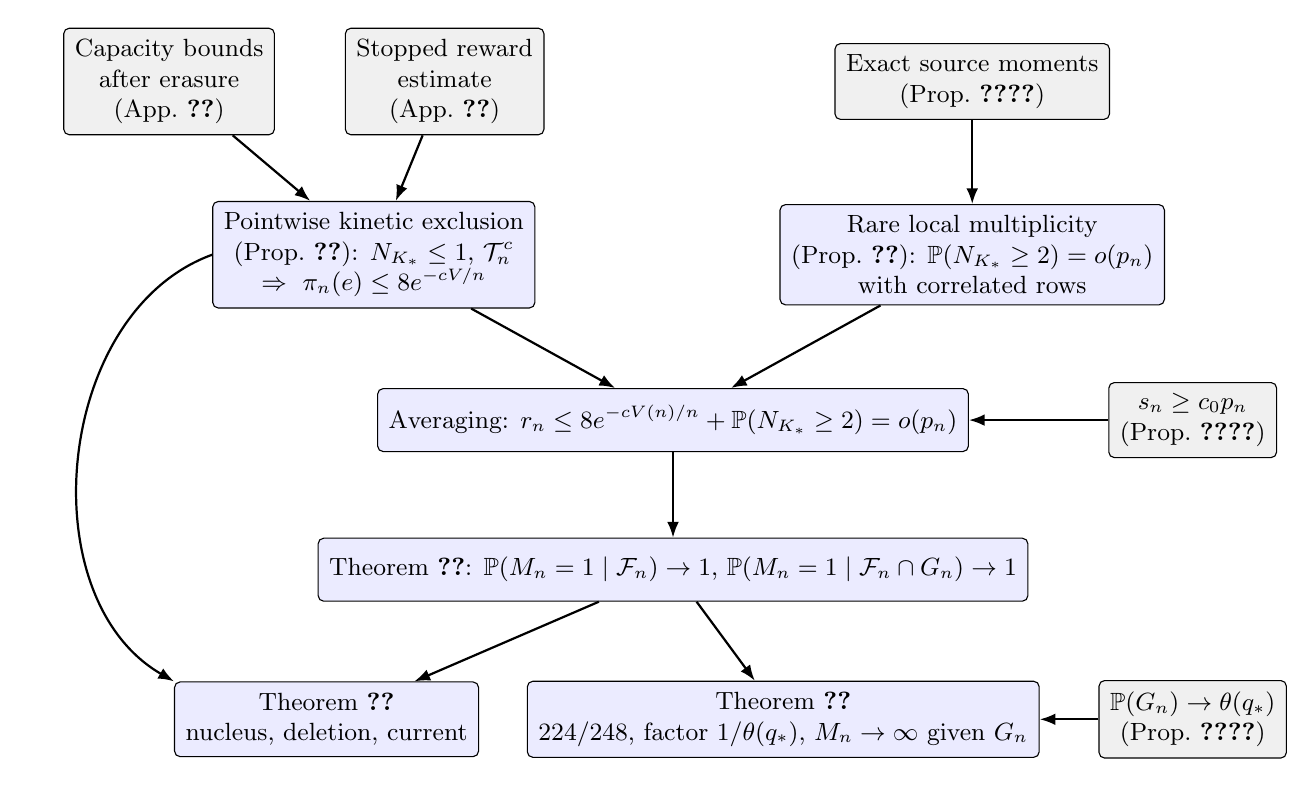
\begin{tikzpicture}[
 box/.style={draw,rounded corners=2pt,align=center,inner sep=4pt,font=\small,minimum height=8mm},
 imp/.style={box,fill=black!6},
 new/.style={box,fill=blue!8},
 arr/.style={-{Latex[length=2mm]},thick}]
 \node[new] (excl) at (0,0) {Pointwise kinetic exclusion\\ (Prop.~\ref{prop:local}): $N_{K_*}\le1$, $\cT_n^c$\\ $\Rightarrow\ \pi_n(e)\le8e^{-cV/n}$};
 \node[new] (mult) at (7.6,0) {Rare local multiplicity\\ (Prop.~\ref{prop:multiple}): $\PP(N_{K_*}\ge2)=o(p_n)$\\ with correlated rows};
 \node[imp] (cap) at (-2.6,2.2) {Capacity bounds\\ after erasure\\ (App.~\ref{app:bounds})};
 \node[imp] (rew) at (0.9,2.2) {Stopped reward\\ estimate\\ (App.~\ref{app:bounds})};
 \node[imp] (mom) at (7.6,2.2) {Exact source moments\\ (Prop.~\ref{prop:imported}\ref{it:moments})};
 \node[new] (avg) at (3.8,-2.1) {Averaging: $r_n\le8e^{-cV(n)/n}+\PP(N_{K_*}\ge2)=o(p_n)$};
 \node[imp] (low) at (10.4,-2.1) {$s_n\ge c_0p_n$\\ (Prop.~\ref{prop:imported}\ref{it:order})};
 \node[new] (main) at (3.8,-4.0) {Theorem~\ref{thm:main}: $\PP(M_n=1\mid\cF_n)\to1$, $\PP(M_n=1\mid\cF_n\cap G_n)\to1$};
 \node[new] (loc) at (-0.6,-5.9) {Theorem~\ref{thm:local}\\ nucleus, deletion, current};
 \node[new] (con) at (5.2,-5.9) {Theorem~\ref{thm:contrast}\\ $224$/$248$, factor $1/\thetaq$, $M_n\to\infty$ given $G_n$};
 \node[imp] (theta) at (10.4,-5.9) {$\PP(G_n)\to\thetaq$\\ (Prop.~\ref{prop:imported}\ref{it:theta})};
 \draw[arr] (cap) -- (excl); \draw[arr] (rew) -- (excl); \draw[arr] (mom) -- (mult);
 \draw[arr] (excl) -- (avg); \draw[arr] (mult) -- (avg); \draw[arr] (low) -- (avg);
 \draw[arr] (avg) -- (main);
 \draw[arr] (main) -- (loc); \draw[arr] (main) -- (con); \draw[arr] (theta) -- (con);
 \draw[arr] (excl.west) to[out=200,in=150] (loc.north west);
\end{tikzpicture}
\caption{Proof map. Shaded boxes are imported from the companion development; blue boxes are proved here. The pointwise exclusion is also used directly for the deletion and current statements.}
\label{fig:map}
\end{figure}

\section{Uniform kinetic exclusion with at most one local incidence}\label{sec:local}

\begin{proposition}[Pointwise kinetic exclusion]\label{prop:local}
Let $e$ be an environment with $N_{K_*}\le1$ and $e\notin\cT_n$, with arbitrary marks and arbitrary assignments outside the $K_*$-rectangle. For every integer $V$ with $V\ge2n/d$ and $n/V\le1/200000$,
\begin{equation}\label{eq:local}
 \pi_{n,V}(e)\le b_n(V):=4e^{-cV/n}+2e^{-d_m^2V/[4n(96011\cdot101+d_m)]}+2e^{-d_o^2V/[4n(96011\cdot101+d_o)]}\le8e^{-cV/n},
\end{equation}
with $d_m=1/200$ and $d_o=1/200000$. Both volume conditions hold under \eqref{eq:volume}.
\end{proposition}
This section gives the mechanism and the numerical budgets. The catalog estimates and the stochastic normalization are in Appendix~\ref{app:bounds}; all bounds concern the original count process \eqref{eq:falling} and remain valid with repeated molecules in the input multiset.

\subsection{Capacity bounds and the case without short incidences}
On $L\le11$ every concentration monomial is bounded, and the mass constraint $\sum_{\ell(z)>K}x_z\le L/K$ converts bounded catalytic coefficients into a capacity bound. Three envelopes, valid on $L\le11$ for a source with no incidence in the $K$-rectangle (Appendix~\ref{app:catalog}), are used repeatedly:
\begin{equation}\label{eq:envelopes}
 b=1936\eps,\qquad t_K=\frac{85184}{K},\qquad \ell_K=1012\eps+\frac{44528}{K},\qquad \beta_K=\frac{550}3\eps+\frac{29040}{K}:
\end{equation}
$b$ bounds the positive basal nonfood-input drift, $t_K$ the positive catalytic nonfood-input drift, $\ell_K$ the drift of loss of a fixed target coordinate of length at most $K/2$, and $\beta_K$ the drift of creation of a fixed nonfood target of length at most $K+2$. All basal pathways remain present; nonlocal catalytic assignments are arbitrary.

If $e$ has no incidence in the $k_0$-rectangle, \eqref{eq:noshort} gives $\pi_n(e)\le4e^{-cV/n}$, the first term of \eqref{eq:local}. Otherwise fix an incidence $(z,r)$ in the $k_0$-rectangle. Since $N_{K_*}\le1$, it is the unique incidence of the larger $K_*$-rectangle, and erasing it leaves a source with no incidence in the $K_*$-rectangle, to which the envelopes \eqref{eq:envelopes} apply with $K=K_*$. Its product has length at most $k_0+2<K_*/2$ and its catalyst length at most $k_0$; these stronger lengths are what the coordinate estimates require.

For $r:u+v\rightleftharpoons p$ put $a=\m(p)-\m(u)-\m(v)$, the nonfood mass gained by one forward firing. By additivity of length there are exactly four cases (Table~\ref{tab:cases}, Figure~\ref{fig:cases}); the fourth is the productive case excluded by $e\notin\cT_n$.

\begin{table}[t]
\centering\small
\begin{tabular}{@{}l>{\raggedright\arraybackslash}p{.30\linewidth}l>{\raggedright\arraybackslash}p{.36\linewidth}@{}}
\toprule
Case & Endpoints and catalyst & $a$ & Controlling observable\\
\midrule
Neutral & all endpoints food, or both inputs nonfood & $0$ & $M$; local increment zero\\
Mixed & one food input, one nonfood input & $1$ or $2$ & $P=M-a\,x_p$; local increment zero in both directions\\
Outsider & food inputs, nonfood product, $z\notin F\cup\{p\}$ & $3$ or $4$ & $P=M+2000\,x_z$; washout of $z$ absorbs the local input\\
Productive & food inputs, nonfood product, $z\in F\cup\{p\}$ & $3$ or $4$ & a one-channel RAF; excluded by $\cT_n^c$\\
\bottomrule
\end{tabular}
\caption{The exhaustive local classification of the unique incidence $(z,r)$, $r:u+v\rightleftharpoons p$. Coincidences of catalyst with an endpoint and equal inputs $u=v$ are included in each case.}
\label{tab:cases}
\end{table}

\begin{figure}[t]
\centering
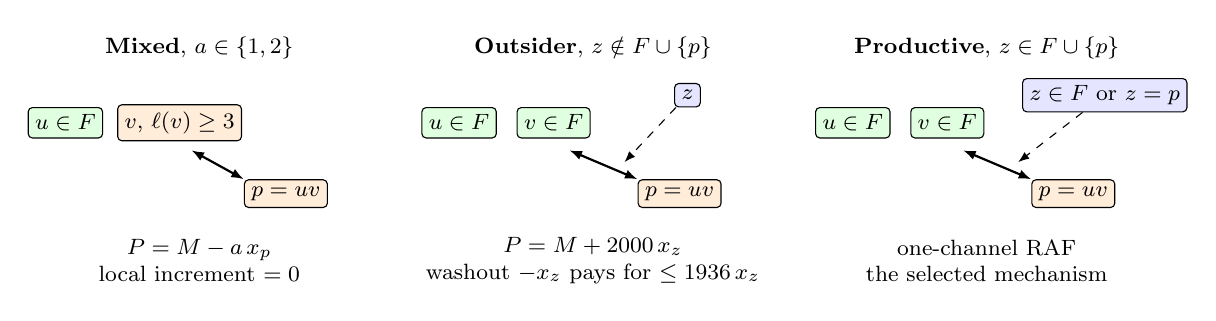
\begin{tikzpicture}[
 mol/.style={draw,rounded corners=1.5pt,inner sep=2.5pt,font=\footnotesize},
 fd/.style={mol,fill=green!12},
 nf/.style={mol,fill=orange!15},
 cat/.style={mol,fill=blue!10},
 lab/.style={font=\footnotesize,align=center},
 arr/.style={{Latex[length=1.6mm]}-{Latex[length=1.6mm]},thick}]
 % panel 1: mixed
 \begin{scope}[shift={(0,0)}]
  \node[lab] at (1.6,1.35) {\textbf{Mixed}, $a\in\{1,2\}$};
  \node[fd] (u) at (-0.1,0.4) {$u\in F$}; \node[nf] (v) at (1.35,0.4) {$v$, $\ell(v)\ge3$};
  \node[nf] (p) at (2.7,-0.5) {$p=uv$};
  \draw[arr] (1.5,0.05) -- (p.north west);
  \node[lab] at (1.6,-1.35) {$P=M-a\,x_p$\\ local increment $=0$};
 \end{scope}
 % panel 2: outsider
 \begin{scope}[shift={(5.0,0)}]
  \node[lab] at (1.6,1.35) {\textbf{Outsider}, $z\notin F\cup\{p\}$};
  \node[fd] (u) at (-0.1,0.4) {$u\in F$}; \node[fd] (v) at (1.1,0.4) {$v\in F$};
  \node[nf] (p) at (2.7,-0.5) {$p=uv$};
  \node[cat] (z) at (2.8,0.75) {$z$};
  \draw[arr] (1.3,0.05) -- (p.north west);
  \draw[-{Latex[length=1.4mm]},dashed] (z) -- (2.0,-0.1);
  \node[lab] at (1.6,-1.35) {$P=M+2000\,x_z$\\ washout $-x_z$ pays for $\le1936\,x_z$};
 \end{scope}
 % panel 3: productive
 \begin{scope}[shift={(10.0,0)}]
  \node[lab] at (1.6,1.35) {\textbf{Productive}, $z\in F\cup\{p\}$};
  \node[fd] (u) at (-0.1,0.4) {$u\in F$}; \node[fd] (v) at (1.1,0.4) {$v\in F$};
  \node[nf] (p) at (2.7,-0.5) {$p=uv$};
  \node[cat] (z) at (3.1,0.75) {$z\in F$ or $z=p$};
  \draw[arr] (1.3,0.05) -- (p.north west);
  \draw[-{Latex[length=1.4mm]},dashed] (z) -- (2.0,-0.1);
  \node[lab] at (1.6,-1.35) {one-channel RAF\\ the selected mechanism};
 \end{scope}
\end{tikzpicture}
\caption{Three of the four local cases (the neutral case has zero nonfood gain and needs no credit). Green: food; orange: nonfood; blue: catalyst. In the mixed case the product credit cancels the channel exactly; in the outsider case the catalyst is neither fed nor produced by the channel, so its washout controls the amplification it could provide.}
\label{fig:cases}
\end{figure}

\subsection{Neutral and mixed channels: a conserved product credit}\label{sec:mixed}
Let $r$ be mixed and set $P=M-a\,x_p$. A forward firing of either local direction of $r$ changes $M$ by $a/V$ and $x_p$ by $1/V$; a reverse firing changes both by the opposite amounts. Hence the local catalytic pathway has \emph{exactly} zero increment of $P$ in both directions. Only net stoichiometry enters, so the identity survives catalyst coincidences and repeated inputs. Since the nonfood input has length at least three and the food input has length $a\le2$, the product satisfies $\ell(p)\ge3+a$, whence $\m(p)-a\ge\tfrac35\m(p)$ and
\begin{equation}\label{eq:credit}
 P\ge\tfrac35M\ge0 ,
\end{equation}
molecule by molecule; the same comparison holds for the modified mass carried out by each washout jump. The local channel may shuttle a lot of material, but its throughput cannot raise $P$.

Let $I_P^+(t)$ be the cumulative positive internal $P$-input on $[0,t]$, normalized by $V$. Since $P(0)=0$, food inflow carries zero $P$-weight, and $P(100)\ge0$, the balance of $P$ together with \eqref{eq:credit} forces, on $\cF_n$,
\begin{equation}\label{eq:mixedneed}
 \tfrac12I_P^+(100)\ \ge\ \tfrac12\cdot\tfrac35E\ >\ \tfrac3{100} .
\end{equation}
On the other side, a positive $P$-increment from any channel other than the two erased local directions is at most its positive ordinary nonfood input plus $a$ times its positive loss of the coordinate $x_p$. Erasure removes only the local pathways, so with $K=K_*$ the envelopes \eqref{eq:envelopes} bound the drift of $\tfrac12I_P^+$ by
\begin{equation}\label{eq:mixedbudget}
 \frac{b+t_{K_*}+2\ell_{K_*}}2=\frac{101178}{25\cdot10^9}=4.04712\cdot10^{-6}<\frac1{200000} .
\end{equation}
The halving keeps every jump of the reward at most $4/V$ (an internal nonfood increment is at most $4/V$, a coordinate increment at most $2/V$). The stopped-reward estimate \eqref{eq:noise} with $d=d_m=1/200$, allowance $1/100$, and horizon $T=101$ shows that, outside an event of probability at most $2e^{-d_m^2V/[4n(96011\cdot101+d_m)]}$,
\[
 \tfrac12I_P^+(100)\le\frac{100}{200000}+\frac1{100}=0.0105<\frac3{100},
\]
contradicting \eqref{eq:mixedneed}. This is the middle term of \eqref{eq:local}. The neutral case is the same argument with $a=0$ and $P=M$, where \eqref{eq:credit} is an equality and the export comparison is even stronger.

\subsection{An outsider catalyst: its washout pays for the amplification}\label{sec:outsider}
Now $u,v\in F$, $\ell(p)>2$, and the catalyst $z$ is a nonfood molecule different from $p$. The local pathway has zero net increment of $x_z$ (the catalyst is returned), and its positive nonfood-input drift is at most $1936\,x_z$: the coefficient is at most $16$, the gain is $a\le4$, and $4x_ux_v\le L^2\le121$. Erasing the incidence does not change the drift of $x_z$, and the nonfood target-creation envelope gives
\begin{equation}\label{eq:outsidercoordinate}
 \cG x_z\le\beta_{K_*}-x_z ,
\end{equation}
where $-x_z$ is washout and the feed contributes nothing to a nonfood coordinate. Take $P=M+2000\,x_z$; since $2000>1936$, the washout of $z$ dominates the local input. To keep the reward jump uniformly small, use the signed reward
\begin{equation}\label{eq:outsiderreward}
 R_o(t)=\frac{B_+(t)+C_+(t)+2000\bigl(x_z(t)-x_z(0)\bigr)}{1001},
\end{equation}
where $B_+$ and $C_+$ are the cumulative positive internal nonfood inputs from basal and from catalytic channels, normalized by $V$. Its drift is at most $F_*/1001$, where
\begin{equation}\label{eq:Fstar}
 F_*=1936\eps+\frac{85184}{K_*}+2000\beta_{K_*}=\frac{37282993}{46875000000},
\end{equation}
because the remaining coefficient of $x_z$ is $1936-2000\le0$. Every jump of \eqref{eq:outsiderreward} has absolute value at most $(4+2000\cdot2)/(1001V)=4/V$.

Initially $M=x_z=0$. Pathwise nonfood mass balance gives $E\le B_+(100)+C_+(100)$ on $\cF_n$, hence $E\le1001R_o(100)$ because $x_z(100)\ge0$. Outside the reward-noise event of allowance $1/100000$, which by \eqref{eq:noise} with $d=d_o$ has probability at most $2e^{-d_o^2V/[4n(96011\cdot101+d_o)]}$,
\begin{equation}\label{eq:outsiderbudget}
 E\le100F_*+\frac{1001}{100000}=\frac{83950361}{937500000}=0.089547051733\ldots<\frac1{10},
\end{equation}
a contradiction with the count event \eqref{eq:output}. This is the last term of \eqref{eq:local}, and Proposition~\ref{prop:local} is proved.

\begin{remark}
Neither a deterministic fluid approximation \cite{kurtz1972relationship,darling2008differential} nor monotonicity of success under added catalysis is used. The finite-copy correction is handled at the level of the falling-factorial propensities and the stopped trajectory law, and the stopping at the mass exit is legitimate because success itself requires a bounded-mass path. The two observables are designed for this reactor: the product credit removes a channel that merely converts existing nonfood material while incorporating a small food fragment, and the washout penalty uses the dilution of a catalyst that is neither fed nor produced by the channel. Neither is a general theorem about arbitrary reaction networks.
\end{remark}

\section{Rare local multiplicity under correlated rows}\label{sec:multiplicity}

\begin{proposition}\label{prop:multiple}
For every fixed integer $K$, $\PP(N_K\ge2)=o(p_n)$.
\end{proposition}
\begin{proof}
Consider a rectangle of $Z$ catalyst rows and $J$ channel columns and let $N$ be the number of its incidences. By \eqref{eq:degreelaw} and uniform sampling without replacement, the probability that a given row hits at least one of the $J$ columns is exactly
\begin{equation}\label{eq:hit}
 h_J=1-\sum_{d=0}^{R_n-1}\omega_{n,d}\,\frac{\binom{R_n-J}{d}}{\binom{R_n}{d}},
\end{equation}
with an impossible binomial coefficient read as zero. Independence of rows gives $\PP(N=0)=(1-h_J)^Z$, and linearity of expectation gives $\EE N=ZJp_n$. The pointwise inequality $\ind_{\{N\ge2\}}\le N-\ind_{\{N\ge1\}}$ yields
\begin{equation}\label{eq:excess}
 \PP(N\ge2)\le ZJp_n-\bigl[1-(1-h_J)^Z\bigr] .
\end{equation}
No independence within a row has been inserted. Two elementary without-replacement bounds hold for $R_n\ge J$:
\begin{equation}\label{eq:hitbounds}
 h_J\ge Jp_n-\Bigl(\frac{J}{R_n-J+1}\Bigr)^2\EE D_z^2,\qquad
 h_J\le\frac{J\,\EE D_z}{R_n-J+1} .
\end{equation}
The lower bound subtracts pairwise overlaps from the sum of the $J$ single-column probabilities; conditional on $D_z=d$, the probability that two given columns are both hit is $d(d-1)/(R_n(R_n-1))\le(d/(R_n-J+1))^2$, and there are $\binom J2\le J^2$ pairs. The upper bound is the single-column union bound with an enlarged denominator. Also $Zh_J-[1-(1-h_J)^Z]\le\binom Z2h_J^2\le Z^2h_J^2$. Substituting in \eqref{eq:excess},
\begin{equation}\label{eq:rectangle}
 \PP(N\ge2)\le Z\Bigl(\frac{J}{R_n-J+1}\Bigr)^2\EE D_z^2+Z^2\Bigl(\frac{J\,\EE D_z}{R_n-J+1}\Bigr)^2 .
\end{equation}
For fixed $Z,J$ multiply by $X_n$. The first term tends to zero by Proposition~\ref{prop:imported}\ref{it:moments} and $R_n/(R_n-J+1)\to1$; the second is $O(X_np_n^2)=o(1)$. Dividing by $X_np_n\to\lambda>0$ proves the claim for that rectangle. For $N_K$ the row and column cardinalities are at most $X_K$ and $R_{K+2}$ and stabilize once $n\ge K+2$, so the conclusion is uniform.
\end{proof}

The cancellation in \eqref{eq:excess} is the essential gain: a first-moment bound alone gives $\PP(N_K\ge2)\le\EE N_K=O(p_n)$, which is of the same order as the success probability. A heavy-tailed row may contain a huge number of assignments; the argument controls that possibility with the actual capped second moment rather than by replacing the row law.

\begin{remark}[The same estimate through pair probabilities]\label{rem:pairs}
For the reader who prefers a second-moment count: for a rectangle of $Z$ rows and $J$ columns, by \eqref{eq:pair} and row independence,
\begin{equation}\label{eq:pairs}
 \EE\binom N2=Z\binom J2q_{2,n}+\binom Z2J^2p_n^2,
\end{equation}
and $\ind_{\{N\ge2\}}\le\binom N2$. Since $q_{2,n}\le\EE D_z^2/(R_n(R_n-1))$, Proposition~\ref{prop:imported}\ref{it:moments} again gives $o(p_n)$. Formula \eqref{eq:pairs} also shows precisely why same-row pairs cannot be replaced by $p_n^2$: the proof succeeds because $q_{2,n}$ is negligible relative to $p_n$, not because assignments become independent.
\end{remark}

\begin{proposition}[Rate]\label{prop:rate}
For every fixed $K$, $\PP(N_K\ge2)/p_n=O_K(n^{-1})$. Consequently the conditional failure probabilities $\PP(\cT_n^c\mid\cF_n)$ and $\PP(U_{n,K}^c\mid\cF_n)$ are $O_K(n^{-1})$.
\end{proposition}
\begin{proof}
Write $a=a_n\ge3/2$, $R=R_n$, $Y=\min(K_z,R)$. Integral comparison gives $\PP(K_z\ge t)\le t^{-a}+t^{1-a}/(a-1)\le3t^{1-a}$ for integers $t\ge1$, using $\zeta(a)\ge1$ and $a-1\ge1/2$. The tail-sum identity for the bounded variable $Y$ gives
\[
 \EE D_z^2\le\EE Y^2=\sum_{t=1}^{R}(2t-1)\PP(K_z\ge t)\le6\sum_{t=1}^Rt^{2-a}\le6R^{3-a}=6R\cdot R^{2/n} .
\]
For $n\ge4$, $R_n\le n2^{n+1}\le2^{2n}$, so $R^{2/n}\le16$ and $\EE D_z^2\le96R_n$; hence $q_{2,n}\le192/R_n$. Since $R_np_n=\EE D_z\sim\lambda n$, dividing \eqref{eq:pairs} by $p_n$ gives a first term $O_{Z,J}(1/n)$ and a second term $O_{Z,J}(p_n)$. The conditional statements follow from the proofs in Sections~\ref{sec:averaging} and \ref{sec:consequences}, whose kinetic exceptions are $O(e^{-n})$.
\end{proof}
The hidden constants depend on the rectangle and are astronomically large for $K=K_*$. The rate neither establishes numerical convergence at accessible $n$ nor permits a cutoff $K(n)$ growing with $n$.

\section{Averaging and the proof of Theorem~\ref{thm:main}}\label{sec:averaging}

Split the finite environment average defining $r_n$ according to whether $N_{K_*}\le1$. On $\{N_{K_*}\le1\}\cap\cT_n^c$ Proposition~\ref{prop:local} applies uniformly in the marks; on the complement bound $\pi_n\le1$. Thus
\begin{equation}\label{eq:average}
 r_n\le b_n(V(n))+\PP(N_{K_*}\ge2) .
\end{equation}
The second term is $o(p_n)$ by Proposition~\ref{prop:multiple}. For the first, \eqref{eq:volume} gives $cV(n)/n\ge3n$ for every $n\ge4$, while Proposition~\ref{prop:imported}\ref{it:moments} gives $p_n\ge e^{-2n}$ eventually, so
\[
 \frac{b_n(V(n))}{p_n}\le8e^{-3n}e^{2n}=8e^{-n}\longrightarrow0 .
\]
This proves \eqref{eq:core}. Since $s_n\ge c_0p_n$ eventually (Proposition~\ref{prop:imported}\ref{it:order}), $\PP(\cT_n^c\mid\cF_n)=r_n/s_n\to0$, and the inclusions \eqref{eq:inclusions} give the first three limits in \eqref{eq:posteriors}. Finally $\PP(\cF_n\cap G_n)=s_n-\PP(\cF_n\cap G_n^c)\ge s_n-r_n$ is eventually positive and of order $p_n$, and $\cF_n\cap G_n\cap\{M_n\ne1\}\subseteq\cF_n\cap\cT_n^c$; dividing proves the last limit. \qed

\section{Proofs of the consequences}\label{sec:consequences}

\subsection{Singleton RAFs and their exact count}
\begin{lemma}\label{lem:singleton}
A single channel $r:u+v\rightleftharpoons p$ forms a RAF $\{r\}$ if and only if $u,v\in F$ and some catalyst of $r$ lies in $F\cup\{p\}$. For every $n\ge4$ there are exactly $224$ productive candidate incidences (of which $192$ have a food catalyst and $32$ are catalyzed by their own product) and exactly $248$ incidences witnessing a singleton RAF; all of them lie in the $4$-rectangle.
\end{lemma}
\begin{proof}
Some direction of $r$ must be enabled from $F$: otherwise $\cl_{\{r\}}(F)=F$, and the RAF condition would put $u,v\in F$, which enables the forward direction. If the reverse direction is enabled, $p\in F$, and by additivity of length $u,v\in F$. Otherwise the forward direction is enabled, again $u,v\in F$. In both cases $\cl_{\{r\}}(F)=F\cup\{p\}$, so the RAF catalyst condition is exactly the one stated. Conversely, the stated conditions place the endpoints and a catalyst in $F\cup\{p\}=\cl_{\{r\}}(F)$.

There are $2\cdot4+4\cdot2=16$ ordered food--food channels with a product of length three and $4\cdot4=16$ dimer--dimer channels with a product of length four; each has $7$ admissible catalysts, six food words and the product, giving $32\cdot7=224$ productive candidates. The remaining singleton channels are the four ordered monomer--monomer channels, whose product is a dimer in $F$; each has six food catalysts, giving $24$ more, and $248$ in total.
\end{proof}

\subsection{Proof of Theorem~\ref{thm:contrast}}
\emph{Part \ref{it:counts}.} For either candidate family, of size $b\in\{224,248\}$, let $Y\le b$ count the candidates present. Then $\EE Y=bp_n$ exactly, and
\[
 0\le\EE Y-\PP(Y\ge1)=\EE[(Y-1)_+]\le(b-1)\PP(Y\ge2)\le(b-1)\PP(N_4\ge2)=o(p_n)
\]
by Proposition~\ref{prop:multiple} with $K=4$. This proves the two asymptotics in \eqref{eq:prefactors}. Next, $s_n\le\PP(\cT_n)+r_n$ gives $\limsup s_n/p_n\le224$, and Proposition~\ref{prop:imported}\ref{it:order} with $q_{0,n}\to6/\pi^2$ gives $\liminf s_n/p_n\ge(6/\pi^2)^6$.

\emph{Part \ref{it:factor}.} By Bayes' identity $\PP(\cF_n\mid G_n)/\PP(\cF_n)=\PP(G_n\mid\cF_n)/\PP(G_n)$, whose numerator tends to one by Theorem~\ref{thm:main} and whose denominator tends to $\thetaq$ by Proposition~\ref{prop:imported}\ref{it:theta}. For the second limit use $\{M_n=1\}\subseteq G_n$, $\PP(M_n=1)=248p_n+o(p_n)$, and $\PP(G_n)\to\thetaq>0$.

\emph{Part \ref{it:diverge}.} First a length bound for small closures.
\begin{lemma}\label{lem:closurelength}
If $S$ contains at most $m$ channels, every word of $\cl_S(F)$ has length at most $K_m=2^{m+1}$.
\end{lemma}
\begin{proof}
Generate $\cl_S(F)$ by adjoining, one at a time, a product or a pair of fragments whenever the corresponding direction of a channel of $S$ is enabled. The initial maximum length is two. A cleavage never increases the maximum. A ligation increases it by at most a factor two, and a ligation that increases it adjoins a product not previously present; each channel has one product, so at most $m$ such increases occur. The final maximum is at most $2\cdot2^m$.
\end{proof}
Now let $S$ be a RAF with $|S|\le m$. Some channel of $S$ is enabled from $F$ before any nonfood word is adjoined: if nothing is ever adjoined, the closure is $F$ and every channel of $S$ has all endpoints in $F$; otherwise the first adjoined word comes from a channel enabled at $F$. If that direction is cleavage, its product is in $F$ and so are its shorter inputs. In every case $S$ contains a channel with both inputs in $F$ and product of length at most four; there are $4+16+16=36$ such channels. That channel has a catalyst in $\cl_S(F)$, hence of length at most $K_m$ by Lemma~\ref{lem:closurelength}. There are at most $36X_{K_m}$ incidences of this form, each of marginal probability $p_n$, so the union bound gives $\PP(M_n\le m)\le36X_{K_m}p_n$ without enumerating RAFs or assuming independence. Dividing by $\PP(G_n)\to\thetaq>0$ gives the second statement. For the third, $\PP(G_n\cap\{M_n>m\})=\PP(G_n)-\PP(M_n\le m)\to\thetaq$, while the numerator $\PP(\cF_n\cap G_n\cap\{M_n>m\})\le\PP(\cF_n\cap\{M_n\ne1\})\le r_n=o(p_n)$ by \eqref{eq:inclusions}. \qed

\subsection{Proof of Proposition~\ref{prop:decomposition}}
Let $Y=\sum_{i\in\cI}\ind_{I_{i,n}}\le224$. Then $\sum_i\PP(\cF_n\cap I_{i,n})=\EE[\ind_{\cF_n}Y]$, whose excess over $\PP(\cF_n\cap\cT_n)=\EE[\ind_{\cF_n}\ind_{\{Y\ge1\}}]$ is $\EE[\ind_{\cF_n}(Y-1)_+]\in[0,223\,\PP(N_4\ge2)]=[0,o(p_n)]$. Adding $r_n=o(p_n)$ gives $s_n=\sum_i\PP(\cF_n\cap I_{i,n})+o(p_n)$, and $\PP(\cF_n\cap I_{i,n})=p_n\alpha_i(n)$ by definition. The posterior identity is Bayes' rule. For \eqref{eq:sizebias}, $\PP(r\in C_z\mid D_z=d)=d/R_n$, so $\PP(D_z=d\mid r\in C_z)=(d/R_n)\omega_{n,d}/p_n=d\,\omega_{n,d}/\EE D_z$, and the conditional mean follows. \qed

\subsection{Proof of Theorem~\ref{thm:local}}
\emph{Part \ref{it:unique}.} Every productive candidate lies in the $4$-rectangle, hence in the $K$-rectangle for $K\ge4$, so
\[
 U_{n,K}^c\subseteq\cT_n^c\cup\{N_K\ge2\} .
\]
Intersect with $\cF_n$, apply \eqref{eq:core} and Proposition~\ref{prop:multiple}, and divide by $s_n\ge c_0p_n$. By Lemma~\ref{lem:singleton} every singleton-RAF witness also lies in the $K$-rectangle, so on $U_{n,K}$ the unique local incidence is the only singleton witness and its channel is the only singleton RAF.

\emph{Part \ref{it:reliable}.} By \eqref{eq:witness}, $H_n\subseteq A_{n,\eta}$ once $24e^{-cV(n)/n}\le1-\eta$, so $\mu_n(A_{n,\eta})\ge q_{0,n}^6p_n$, which gives the lower prefactor. Next, since $\pi_n\ge\eta$ on $A_{n,\eta}$,
\begin{equation}\label{eq:reliableineq}
 \eta\,\mu_n(\cT_n^c\cap A_{n,\eta})\le\EE_{\mu_n}[\pi_n\ind_{\cT_n^c}]=r_n=o(p_n),
\end{equation}
and likewise $\mu_n(U_{n,K}^c\cap A_{n,\eta})\le\mu_n(\cT_n^c\cap A_{n,\eta})+\mu_n(N_K\ge2)=o(p_n)$; dividing by $\mu_n(A_{n,\eta})\ge q_{0,n}^6p_n$ gives both conditional limits. Finally $\mu_n(A_{n,\eta})\le\mu_n(\cT_n)+\mu_n(\cT_n^c\cap A_{n,\eta})\le224p_n+o(p_n)$. The fixed threshold matters: the bound divides by $\eta$.

\emph{Part \ref{it:delete}.} On $U_{n,K_*}$ every incidence of the $K_*$-rectangle is the erased one, so the erased source has no incidence in the $K_*$-rectangle and a fortiori none in the $k_0$-rectangle. The erased reactor has the same rate caps and the same food-only initial state, so \eqref{eq:noshort} applies to it and gives \eqref{eq:delete}. The two typicality statements are Parts \ref{it:unique} and \ref{it:reliable}, and on $A_{n,\eta}$ the original success probability is at least $\eta$.

\emph{Part \ref{it:current}.} Fix $e\in U_{n,K_*}$ with its unique local incidence $(z,r)$. Let $C_{\oth,+}$ be the positive nonfood-input reward of all catalytic pathways other than the two local directions of $(z,r)$, on the \emph{original} reactor. Its drift at any population equals the positive catalytic nonfood-input drift of the erased source at the same population, because the reward is simply zero on the two local channels; this is an identity between instantaneous rate sums and not a transfer between trajectory laws. Hence its drift is at most $t_{K_*}=85184/K_*$ on $L\le11$, while $B_+$ has drift at most $b$. Both rewards have jumps in $[0,4/V]$ and satisfy the variance bound \eqref{eq:variance} under the original total rate. Apply \eqref{eq:noise} to each with $d=1/200$, allowance $1/100$, $T=101$; a union bound gives an exceptional probability at most $4e^{-cV/n}$, uniform over environments in $U_{n,K_*}$. On the complementary bounded-mass paths
\begin{equation}\label{eq:currentbudget}
 B_+(100)+C_{\oth,+}(100)\le100\Bigl(1936\eps+\frac{85184}{10^{12}}\Bigr)+\frac2{100}=0.0203957184<\frac1{40} .
\end{equation}
Pathwise nonfood mass balance with $M(0)=0$ reads
\[
 M(100)+\frac{W((0,100])}V=J_\loc(100)+J_\oth(100)+J_{\rm basal}(100),
\]
where the three signed inputs are the local, other-catalytic, and basal contributions. Since $M(100)\ge0$, $W((0,100])\ge W((1,100])$, and signed inputs are at most their positive parts,
\[
 J_\loc(100)\ge E-B_+(100)-C_{\oth,+}(100)>E-\tfrac1{40}>\tfrac34E>\tfrac3{40}
\]
on $\cF_n$ outside the exceptional event. The incidence is determined by the environment, so no union over candidate incidences is needed. Averaging over $U_{n,K_*}$ and adding $\PP(\cF_n\cap U_{n,K_*}^c)=o(p_n)$ gives a total exception of $o(p_n)$; divide by $s_n\ge c_0p_n$. \qed

\section{Discussion and scope}\label{sec:discussion}

\paragraph{Selection by an operational event.}
The same sampler gives three different answers to ``what does a typical environment contain'', depending on the conditioning (Table~\ref{tab:questions}). RAF existence has a positive limit $\thetaq$, and under that conditioning the minimum RAF is large: $M_n\to\infty$ in probability, although subexponentially. Singleton RAFs have probability $248p_n+o(p_n)$, exponentially small. Productive output has probability $\Theta(p_n)$, and conditioning on it selects, with probability tending to one, an environment containing one of the $224$ short productive incidences, exactly one incidence in a huge fixed neighbourhood, and nothing else short. The selection is by the operational event, not by an alteration of the chemistry or of the RAF definition, and the strength of the conclusion is exactly that the exceptional set is $o(p_n)$ rather than $o(1)$.

\begin{table}[t]
\centering\small
\begin{tabular}{@{}p{.50\linewidth}p{.44\linewidth}@{}}
\toprule
Question & Answer proved here\\
\midrule
What does a typical successful realization contain? & A productive singleton incidence, unique in the $K_*$-rectangle, with probability $\to1$ (Theorems~\ref{thm:main}, \ref{thm:local}\ref{it:unique}).\\[2pt]
Is the singleton only a coexisting structural certificate? & No: deleting it makes success exponentially unlikely, and it supplies more than $\tfrac34$ of the measured export (Theorem~\ref{thm:local}\ref{it:delete},\ref{it:current}).\\[2pt]
Do ordinary RAF-containing environments contain a singleton? & Almost never: $\PP(M_n=1\mid G_n)\to0$ and $M_n\to\infty$ in probability given $G_n$ (Theorem~\ref{thm:contrast}).\\[2pt]
Must every successful realization contain a singleton, or any RAF? & Not proved; the theorem is about typicality.\\[2pt]
Does every eligible singleton guarantee success? & Not proved; ``productive'' names a structural type.\\[2pt]
Is the rest of the chemistry inactive in a successful run? & Not claimed; localization concerns a fixed rectangle and one net-input observable.\\[2pt]
Must a one-channel RAF copy its catalyst? & No; $192$ of the $224$ candidates have a food catalyst.\\
\bottomrule
\end{tabular}
\caption{What the theorems decide and what they leave open.}
\label{tab:questions}
\end{table}

\paragraph{The mechanism.}
The kinetic exclusion is a resource and startup constraint made quantitative by two observables. A mixed channel can incorporate food while cycling existing nonfood material, but it cannot create the credited mass needed to initialize that material; the product credit $M-a\,x_p$ records this as an exact cancellation. An outsider catalyst can accelerate food conversion, but in a locally sparse environment it is neither fed nor made by the channel it accelerates, and its washout removes it faster than it can pay for itself; the penalty $M+2000\,x_z$ records this with the margin $2000-1936$. A productive singleton escapes both obstructions because its catalyst is either supplied by the feed or made by the same food-enabled channel. A large catalytic degree by itself does not defeat the mass-tail bound: the envelopes \eqref{eq:envelopes} allow every nonlocal assignment. This is why the result needs no sparsity of the global network and no bound on the number of catalysts a molecule can have.

\paragraph{A transferable pattern.}
The structure of the argument is not specific to the observables. Let $\mu_n$ be environment laws, $\pi_n\in[0,1]$ success probabilities, $T_n$ candidate events, and $N_n$ nonnegative integer local counts, and suppose for some scale $p_n>0$: (1) $\int\pi_n\,\dd\mu_n\ge c_0p_n$ eventually; (2) $\pi_n\le b_n=o(p_n)$ on $T_n^c\cap\{N_n\le1\}$; (3) $\mu_n(N_n\ge2)=o(p_n)$. Then $\mu_n^{\rm succ}(T_n^c)\le(b_n+\mu_n(N_n\ge2))/(c_0p_n)\to0$, and if also $\mu_n(A_{n,\eta})\ge c_\eta p_n$ the reliable-environment conclusion follows as in \eqref{eq:reliableineq}. In the present paper (1) is the constructive witness, (2) the two observables, and (3) the excess-count estimate; each is replaced separately if the source or reactor changes. An independent-row source with common marginal $p_n\to0$ and same-row pair probability $q_{2,n}=o(p_n)$ satisfies (3) automatically by \eqref{eq:pairs}, but that alone supplies neither (1) nor (2).

\paragraph{The screen interpretation and its limits.}
The $224$ candidate incidences form an asymptotically sensitive screen among successful realizations: the conditional false-negative probability tends to zero, at rate $O(1/n)$ by Proposition~\ref{prop:rate}. The theorems do not give a low false-positive rate, a sufficiency test for any candidate, or the leading success constant; Proposition~\ref{prop:decomposition} states exactly what is missing. The volume envelope \eqref{eq:volume} is a sufficient condition of the proof method, chosen so that $e^{-cV(n)/n}=o(p_n)$ with ample slack; it is not a lower bound on physically necessary reactor volume, and the huge cutoffs $k_0$, $K_*$ prevent any reading of the result as a calibrated laboratory threshold.

\paragraph{Open questions.}
Exceptional productive systems with large minimum RAFs, or with no RAF at all, are compatible with every theorem here. Establishing a productive $16$-channel catalytic cycle at $n=4$, a productive acyclic organization without any RAF, a uniform theorem for arbitrary finite catalytic support, a smaller sufficient volume, or the limits of the $\alpha_i(n)$ each requires an argument beyond this paper. None alters the conditional assertion proved: in the stated source and volume regime, and after conditioning on productive output, the minimum RAF has size one and the one-channel RAF is the mechanism.

\appendix
\section{Capacity, target, and stopped-reward bounds}\label{app:bounds}

Write $Q=\sum_zx_z$; then $Q\le L$ and $\sum_{\ell(z)>K}x_z\le L/K$. For every count propensity $(N_z)_h/V^h\le x_z^h$, so upper drift bounds follow from nonnegative concentration monomials without any continuum approximation.

\subsection{Catalog counting and coordinate bounds}\label{app:catalog}
The map from a channel to its product word and left-input length is injective. A fixed target $q$ is produced by at most one ligation for each ordered pair of reactants, and by the cleavage of any fixed parent at most twice (both fragments may equal $q$). The unit-coefficient positive target-creation sum is therefore at most
\begin{equation}\label{eq:creation}
 Q^2+2Q ;
\end{equation}
the multiplicity two is real and cannot be removed by treating the fragments as a set. Losses of a target are bounded by counting its occurrences in the two input positions and the product position, which gives the basal loss bound $4\eps(2L^2+L)\le1012\eps$ at $L\le11$.

For a nonfood target the basal creation bound sharpens. Let $A=\sum_{\ell(z)=1}x_z$. Monomer--monomer pairs cannot make a nonfood word, so forward creation is at most $Q^2-A^2$; since $L\ge2Q-A$ and $(Q-2A)^2\ge0$,
\[
 3(Q^2-A^2)\le(2Q-A)^2\le L^2 .
\]
A parent cleaving to a nonfood target has length at least four, so the two-occurrence bound makes reverse creation at most $L/2$. Multiplying by $4\eps$,
\begin{equation}\label{eq:nonfoodcreation}
 4\eps\Bigl(\frac{L^2}3+\frac L2\Bigr)\le\frac{550}3\eps .
\end{equation}
This sharpening is what makes the outsider budget \eqref{eq:outsiderbudget} close; the crude $Q^2+2Q$ would not.

For catalytic bounds in a source with no incidence in the $K$-rectangle, split channels by whether the product length is at most $K+2$. A short-product channel has catalyst length greater than $K$, so the mass-tail bound applies to the catalyst sum; a long product created by cleavage of a specified short target has a parent of small concentration; a long product consuming a target of length at most $K/2$ in its forward direction has another input of length greater than $K/2$. Applying the two positional multiplicities, \eqref{eq:creation}, and the coefficient cap $16$:
\begin{center}\small
\begin{tabular}{@{}lll@{}}
\toprule
Quantity, after local erasure & Envelope at mass $L$ & At $L\le11$\\
\midrule
Positive catalytic nonfood input & $64L^3/K$ & $85184/K$\\
Loss of a target with $\ell(q)\le K/2$ & $(16L^2+32L^3)/K$ & $44528/K$\\
Creation of a target with $2<\ell(q)\le K+2$ & $(16L^3+64L^2)/K$ & $29040/K$\\
\bottomrule
\end{tabular}
\end{center}
For the first row write $Q_K=\sum_{\ell(z)>K}x_z$ and $F_0=\sum_{f\in F}\ell(f)x_f$. The nonfood gain of a ligation is at most the food weight among its two inputs. For each food input position, absence of a local incidence forces either the catalyst or the other input to have length greater than $K$; summing over the two positions and the two alternatives bounds the unit-coefficient food-input sum by $4Q_KF_0Q\le4L^3/K$, and the cap $16$ gives $64L^3/K$. The second row separates product loss with a long catalyst ($16L^2/K$) from target consumption with a long catalyst or a long partner ($32L^3/K$). The third separates long-catalyst forward production ($16L^3/K$) from cleavage contributions, whose two target occurrences and long-parent-or-long-catalyst partition give $64L^2/K$. These envelopes may count overlapping contributions more than once; none uses a bound on catalytic degree. Positive basal nonfood input is at most $16\eps L^2\le1936\eps$. In \eqref{eq:outsidercoordinate} the washout supplies $-x_z$, the feed contributes zero, and the local incidence has zero net $z$-increment; in \eqref{eq:mixedbudget} the target $p$ has length at most $k_0+2<K_*/2$ as the loss bound requires.

\subsection{The stopped reward estimate and the physical time window}\label{app:reward}
The following estimate is proved for the actual jump kernel in the formal development (\lean{physical_marked_reward_two_sided_interval_tail}). Let $\rho(N,j)$ be a reward attached to the jump of type $j$ from population $N$ with $|\rho|\le n/V$, and suppose that whenever $L\le11$,
\begin{equation}\label{eq:variance}
 \sum_j\lambda_j(N)\rho(N,j)^2\le\frac{384000+11n}{V} .
\end{equation}
If $d>0$, $T\ge0$, and $d+n/V\le h$, then the probability that the absolute compensated reward exceeds $h$ anywhere on the physical interval $[0,T]$, stopped at the first exit from $L\le11$, is at most
\begin{equation}\label{eq:noise}
 2\exp\Bigl(-\frac{d^2V}{4n(96011T+d)}\Bigr) .
\end{equation}
The statement covers the unfinished holding interval at the observation time, not only jump epochs; $n/V$ is the interval-boundary allowance. The proof compensates each marked jump by its conditional rate, uses the exponential waiting-time law and $e^u-1-u\le u^2$ for $|u|\le1$ to bound the logarithmic transform by the accumulated quadratic rate, stops the resulting nonnegative exponential supermartingale at the first crossing, and uses both signs; passing through finite jump prefixes and the censored last waiting time, and identifying the countable-prefix formulation with the physical event through nonexplosion, gives \eqref{eq:noise}. General martingale tail bounds \cite{freedman1975tail} and Markov-chain approximation results \cite{darling2008differential} provide context; the constants and the interval adapter are checked for this kernel. Censoring at the mass exit is essential, and it is legitimate because the output event itself supplies the bounded-mass path.

All rewards used in Sections~\ref{sec:mixed}, \ref{sec:outsider}, and \ref{sec:consequences} have absolute jump at most $4/V\le n/V$. On $L\le11$ the total physical rate, with basal coefficients at most one and catalytic coefficients at most $16$, is at most $24000V$, so $\sum_j\lambda_j\rho_j^2\le24000V(4/V)^2=384000/V$, verifying \eqref{eq:variance}. For the signed outsider reward the coordinate term includes washout, and its jump estimate covers external channels as well. For the masked reward $C_{\oth,+}$ of Theorem~\ref{thm:local}\ref{it:current}, setting two rewards to zero leaves the variance argument valid under the original law.

The proofs use $T=101$ to cover the horizon $100$ and its censored interval representation. The volume envelope gives $n/V\le1/200000$, the scale used in \eqref{eq:noshort}, and the margins $d_m+n/V\le1/100$ and $d_o+n/V\le1/100000$. Since
\[
 c\le\frac{d_m^2}{4(96011\cdot101+d_m)},\qquad c\le\frac{d_o^2}{4(96011\cdot101+d_o)},
\]
the three terms of \eqref{eq:local} are bounded by $8e^{-cV/n}$, and the current-attribution exception by $4e^{-cV/n}$.

\section{Formal concordance and reproducibility}\label{app:formal}

The Lean development is a single project pinned to \texttt{leanprover/lean4:v4.30.0} with Mathlib at commit \texttt{c5ea00351c28e24afc9f0f84379aa41082b1188f}. The reactor namespace is \lean{RandomViability}; it imports the source namespace \lean{PowerLawSmallRAF}, and both use the configuration weight \lean{sourcePowerLawConfigWeight}, which is \eqref{eq:weight}. The productive event is \lean{physicalOutputEvent} (mass at most $11V$ through time $100$ and windowed export reward above $1/10$ on $(1,100]$), the joint probability \lean{outputJointProbability} (source average, uniform mark average, and trajectory law), the incidence probability \lean{productiveSourceIncidence} $=p_n$, the noise rate \lean{markedNoiseRate} $=c$, the cutoffs \lean{collectiveUpperCutoff} $=k_0$ and \lean{singleIncidenceCutoff} $=K_*$, and the volume envelope \lean{collectiveMinimalVolume} $=10^{60}(n+1)^2$. The productive-incidence predicate is \lean{ProductiveSingletonIncidence}, the RAF event \lean{anySourceRAF}, and the singleton event \lean{hasSingletonRAF}.

Two strict verification receipts accompany the paper. Each records exit code zero, warnings treated as errors, no \texttt{sorry}, the axioms \texttt{Classical.choice}, \texttt{Quot.sound}, and \texttt{propext} only, and the SHA-256 of every compiled source in the import closure ($407$ and $408$ modules).

\begin{center}\small
\begin{tabular}{@{}>{\raggedright\arraybackslash}p{.34\linewidth}>{\raggedright\arraybackslash}p{.62\linewidth}@{}}
\toprule
Paper statement & Lean declaration (file in \texttt{proofs/RandomViability/} unless stated)\\
\midrule
Prop.~\ref{prop:local}, pointwise exclusion & \lean{physical_output_upper_at_most_one_local} (\lean{LocalOutputExclusion.lean}); hypotheses: no productive incidence, at most one incidence in the $K_*$-rectangle, food-only initial state, the rate caps, and the volume margins\\[2pt]
Prop.~\ref{prop:multiple}, source multiplicity & \lean{two_local_incidence_mass_div_incidence_tendsto_zero} (\lean{LocalMultiplicity.lean}), for every fixed cutoff\\[2pt]
Thm.~\ref{thm:main}, \eqref{eq:core} & \lean{output_without_productive_singleton_relative_tendsto_zero} (\lean{SingletonDominance.lean}); root receipt on \lean{Remark34.lean}, source SHA-256 \texttt{2fec12f3\ldots}, 80.4 s\\[2pt]
Lemma~\ref{lem:singleton}, first sentence ($\Leftarrow$) & \lean{productive_incidence_singleton_isRAF} (\lean{ProductiveSingletonRAF.lean})\\[2pt]
Thm.~\ref{thm:main}, $\PP(M_n=1\mid\cF_n\cap G_n)\to1$ & \lean{remark34_no_singleton_given_productive_raf_tendsto_zero} with \lean{singleton_raf_minimum_card} (\lean{Remark34.lean}); the denominator is output jointly with RAF existence\\[2pt]
Thm.~\ref{thm:main}, output-only posteriors & \lean{no_RAF_given_output_tendsto_zero}, \lean{no_singleton_RAF_given_output_tendsto_zero} (\lean{PublicationFollowups.lean}); receipt source SHA-256 \texttt{c370c68c\ldots}, 217.5 s\\[2pt]
Thm.~\ref{thm:local}\ref{it:delete}, pointwise bound \eqref{eq:delete} & \lean{deleted_unique_incidence_output_upper} (\lean{PublicationFollowups.lean}), for the erased source \lean{eraseLocalIncidence}\\[2pt]
Prop.~\ref{prop:imported}\ref{it:order} & \lean{output_joint_probability_theta} (\lean{OutputJointLimit.lean})\\[2pt]
Prop.~\ref{prop:imported}\ref{it:theta} & \lean{PowerLawSmallRAF.source_RAF_probability_tendsto} (\lean{proofs/PowerLawSmallRAF/Main.lean}), limit \lean{(staticSurvival sourceCriticalOpenness).toReal}, positive by \lean{sourceCriticalSurvival_pos}\\[2pt]
Appendix~\ref{app:reward}, \eqref{eq:noise} & \lean{physical_marked_reward_two_sided_interval_tail} (\lean{MarkedRewardInterval.lean})\\
\bottomrule
\end{tabular}
\end{center}

\paragraph{Conventional proofs.}
Lemma~\ref{lem:singleton} (the counts), Theorem~\ref{thm:local}\ref{it:unique}, \ref{it:reliable}, the typicality parts of \ref{it:delete}, and \ref{it:current}, Theorem~\ref{thm:contrast} in full, Proposition~\ref{prop:decomposition}, and Proposition~\ref{prop:rate} are proved in the text and have no separate terminal Lean export. The current-attribution proof verifies the reward hypotheses in the original law explicitly rather than transferring a concentration estimate between reactors. The Lean statements are event-level: $M_n$ is not a formal random variable, and the minimum-cardinality reading is the elementary interpretation of \lean{singleton_raf_minimum_card} on the finite configuration space.

\paragraph{Reproduction.}
The exact-arithmetic script \texttt{check\_paper.py} distributed with the source replays every number printed in this paper: the catalog counts $30$, $68$, $36$, $224$, $248$, $192$, $32$; the envelopes \eqref{eq:envelopes}; the budgets \eqref{eq:mixedbudget}, \eqref{eq:outsiderbudget}, \eqref{eq:currentbudget}; the noise constants and the inequalities $c\le d_m^2/[4(96011\cdot101+d_m)]$, $cV(n)/n\ge3n$; and the bounds in Proposition~\ref{prop:rate}. It performs no simulation. No numerical simulation is used as evidence anywhere in this paper. Proof verification uses the repository bridge, which sets the Mathlib working directory, treats warnings as errors, and writes the receipts named above; no dependency update is required.

\bibliographystyle{plainnat}
\bibliography{refs}

\end{document}
